\subsection{Exercises}
Find the radian measure of the angle with the given degree measurements. 

\begin{description}
\item [1.]   
%TCIMACRO{\TeXButton{Start Two Columns}{\columnsep =30pt
% \begin {multicols}{2}}}%
%BeginExpansion
\columnsep =30pt
\begin {multicols}{2}
%EndExpansion
 $36 \mbox{{\ensuremath{{}^\circ}}}$ 

\item [3.]
$ -480 \mbox{{\ensuremath{{}^\circ}}}$ 
%TCIMACRO{\TeXButton{End Two Columns}{\end {multicols}}}%
%BeginExpansion
\end {multicols}
%EndExpansion
 

\item [5.]
%TCIMACRO{\TeXButton{Start Two Columns}{\columnsep =30pt
% \begin {multicols}{2}}}%
%BeginExpansion
\columnsep =30pt
\begin {multicols}{2}
%EndExpansion
 $60 \mbox{{\ensuremath{{}^\circ}}}$ 

\item [7.]
$ -135 \mbox{{\ensuremath{{}^\circ}}}$ 
%TCIMACRO{\TeXButton{End Two Columns}{\end {multicols}}}%
%BeginExpansion
\end {multicols}
%EndExpansion
 \end{description}

Find the degree measure of the angle with the given radian measure. 


\begin{description}

%TCIMACRO{\TeXButton{Start Two Columns}{\columnsep =30pt
% \begin {multicols}{2}}}%
%BeginExpansion
\columnsep =30pt
\begin {multicols}{2}\item [9.]
%EndExpansion
 $\frac{3 \pi }{4}$ 

\item [11.] $\frac{5 \pi }{6}$ 
%TCIMACRO{\TeXButton{End Two Columns}{\end {multicols}}}%
%BeginExpansion
\end {multicols}
%EndExpansion
 

\item [13.]
%TCIMACRO{\TeXButton{Start Two Columns}{\columnsep =30pt
% \begin {multicols}{2}}}%
%BeginExpansion
\columnsep =30pt
\begin {multicols}{2}
%EndExpansion
 $ -1.5$ 

\item [15.] $ -\frac{\pi }{12}$ 
%TCIMACRO{\TeXButton{End Two Columns}{\end {multicols}}}%
%BeginExpansion
\end {multicols}
%EndExpansion
 

\item [41.]
%TCIMACRO{\TeXButton{Start Two Columns}{\columnsep =30pt
% \begin {multicols}{2}}}%
%BeginExpansion
\columnsep =30pt
\begin {multicols}{2}
%EndExpansion
 Find the length of the arc $s$ in the figure. \\\relax The radius is $5$. 

\item    
\setlength\fboxrule{0in}\setlength\fboxsep{0.2in}\fcolorbox[HTML]{000000}{FFFFFF}{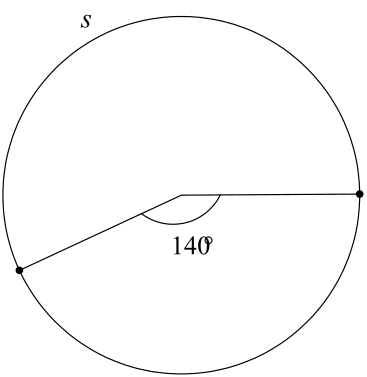
\includegraphics[ width=1.8057in, height=1.8507in,]{L4SZ281B}
}


\item [43.] Find the radius $r$ of the circle in the figure. 

\item    
\setlength\fboxrule{0in}\setlength\fboxsep{0.2in}\fcolorbox[HTML]{000000}{FFFFFF}{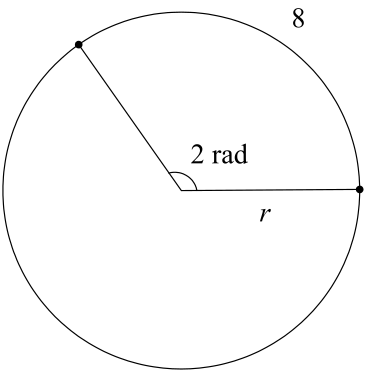
\includegraphics[ width=1.8196in, height=1.8438in,]{L4SZ281C}
}
%TCIMACRO{\TeXButton{End Two Columns}{\end {multicols}}}%
%BeginExpansion
\end {multicols}
%EndExpansion
 

\item [45.]
Find the length of an arc that subtends a central angle of $2 \mbox{rad}$ in a circle of radius 2mi. 

\item [47.]
An arc of length $100 \mbox{m}$ subtends a central angle in
a circle of radius $50 \mbox{m}$. Find the measure of $\theta $\ in degrees and in radians. 

\item [49.]
Find the radius of the circle if an arc of length $6 \mbox{m}$ on the circle subtends a central angle of $\pi /6$ rad. 

\item [51] Pittsburgh, Pennsylvania
and Miami, Florida lie approximately on the same meridian. Pittsburgh has a latitude of $40.5 \mbox{{\ensuremath{{}^\circ}}}$ N and Miami is $25.5 \mbox{{\ensuremath{{}^\circ}}}$ N. Find the distance between these two cities. (The
radius of the earth is $3960 \mbox{mi}\text{.}$) 

\item [53.] Find the distance
the earth travels in one day in its path around the sun. Assume the year has $365$ days and that the path of the earth around the sun is a circle of radius $93$ million miles. 

\item [55.] Find
the distance along an arc on the surface of the earth that subtends an angle of 1 minute. ($1$ minute = $\frac{1}{60}$ degree). This distance is called a nautical mile. The
radius of the earth is $3960 \mbox{mi}\text{.}$ 

\item [57.] Find the area
of a sector with a central angle $1 \mbox{rad}$ in a circle of radius $10 \mbox{m}$. 

\item [59.]
The area of a sector of a circle with a central angle of $2 \mbox{rad}$ is $16 \mathrm{m}^{2}$. Find the radius of the circle. 

\item [61.]
The area of the circle is $72 cm^{2}$. Find the area of a sector of the circle that subtends an angle of $\pi /6 \mbox{rad}\text{.}$ \\

\subsection{Exercises}
\begin{description}
	\item [1.]  Find the exact value of $\sin  \theta $, $\cos  \theta $ and $\tan  \theta $ of the angle $\theta $ in the triangle. \\
	
	\setlength\fboxrule{0in}\setlength\fboxsep{0.2in}\fcolorbox[HTML]{000000}{FFFFFF}{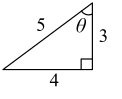
\includegraphics[ width=1.1632in, height=0.9548in,]{L4SZ281K}	}
	
	\item [3.]  Find the angle $\theta$  
	\setlength\fboxrule{0in}\setlength\fboxsep{0.2in}\fcolorbox[HTML]{000000}{FFFFFF}{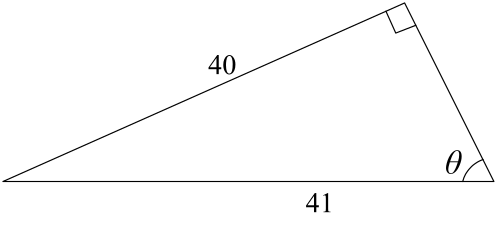
\includegraphics[ width=2.8003in, height=1.2756in,]{L4SZ281L}	}
	
	\item [5.] Find the angle $\theta$
	\setlength\fboxrule{0in}\setlength\fboxsep{0.2in}\fcolorbox[HTML]{000000}{FFFFFF}{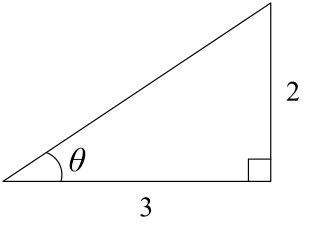
\includegraphics[ width=1.9562in, height=1.3932in,]{L4SZ281M}	}
\end{description}
\clearpage
Find the side length labelled $x$ for 10,11, and 13. 


\begin{description}
	
	\columnsep =30pt
	\begin {multicols}{2}
	\item [10.]       
	\setlength\fboxrule{0in}\setlength\fboxsep{0.2in}\fcolorbox[HTML]{000000}{FFFFFF}{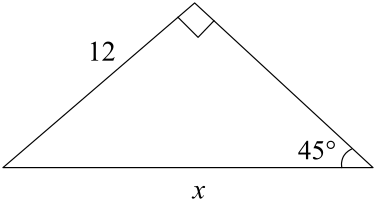
\includegraphics[ width=2.1698in, height=1.2254in,]{L4SZ281N}	}
	
	
	\item [11.]    
	\setlength\fboxrule{0in}\setlength\fboxsep{0.2in}\fcolorbox[HTML]{000000}{FFFFFF}{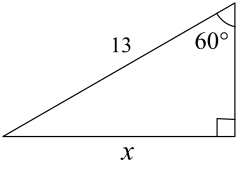
\includegraphics[ width=1.7348in, height=1.2462in,]{L4SZ281O}	}
	
	\item [13.]
	\setlength\fboxrule{0in}\setlength\fboxsep{0.2in}\fcolorbox[HTML]{000000}{FFFFFF}{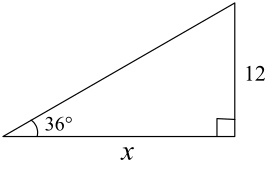
\includegraphics[ width=1.996in, height=1.2289in,]{L4SZ281P}	}
	\item [29.]   Solve the triangle 
	
	\setlength\fboxrule{0in}\setlength\fboxsep{0.2in}\fcolorbox[HTML]{000000}{FFFFFF}{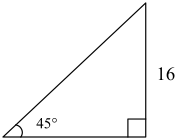
\includegraphics[ width=2.0055in, height=1.4909in,]{L4SZ281Q}	}
	
	
	\item [31.]    Solve the triangle 
	\setlength\fboxrule{0in}\setlength\fboxsep{0.2in}\fcolorbox[HTML]{000000}{FFFFFF}{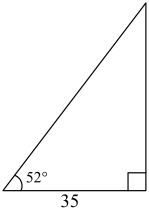
\includegraphics[ width=1.5843in, height=2.3065in,]{L4SZ281R}	}
	\end {multicols}
	
	
	\item [35.]
	The angle of elevation to the top of the Empire State Building in New York is found to be $11 \mbox{{\ensuremath{{}^\circ}}}$ from the ground at a distance of $1 \mbox{mi}$ from the base of the building. Using this information,
	find the height of the Empire State Building. 
	
	\item [35.]
	A laser beam is to be directed towards the centre of the moon but the beam strays $0.5 \mbox{{\ensuremath{{}^\circ}}}$ from its intended path. 
	
	\item [(a)]
	How far has the beam diverged from its assigned target when it reaches the moon? (The distance of the earth
	to the moon is $240$ $000 \mbox{mi}\text{.}$) 
	
	\item [(b)] The radius
	of the moon is about $1000 \mbox{mi}$. Will the beam strike the moon? 
	
	\item [39.]
	A $20 \mbox{ft}$ ladder leans against a building so that the angle between the ground and the ladder is $72 \mbox{{\ensuremath{{}^\circ}}}$. How high does the ladder reach on the building?
	
	
	\item [42.] A $96 \mbox{ft}$ tree casts a shadow that is $120 \mbox{ft}$ long. What is the angle of elevation of the sun?
	
	
	\item [43.] a man is lying on the beach, flying a kite. He
	holds the end of the kite string at ground level, and estimates that the angle of elevation of the kite to be $50 \mbox{{\ensuremath{{}^\circ}}}$. If the string is $450 \mbox{ft}$ long, how high is the kite above the ground? 
	
	\item [45.]
	A water tower is located $325 \mbox{ft}$ from a building. From a window in the building
	it is observed that the angle of elevation to the top of the tower is $39 \mbox{{\ensuremath{{}^\circ}}}$ and the angle of depression to the bottom of the tower is $25 \mbox{{\ensuremath{{}^\circ}}}$. How tall is the tower? How
	high is the window? 
	
	\item [46.] An airplane is flying at an
	elevation of $5150 \mbox{ft}$ directly above a straight highway. Two motorists
	are driving cars on the highway on opposite sides of the plane and the angle of depression to one car is $35 \mbox{{\ensuremath{{}^\circ}}}$ and to the other is $52 \mbox{{\ensuremath{{}^\circ}}}$. How far apart are the cars? 


\item [51.] Find the area of a triangle
with sides of length $7$ and $9$ and included angle $72 \mbox{{\ensuremath{{}^\circ}}}$. 

\item [53.]
A triangle has an area of $16 in^{2}\text{,}$ and two of the sides of the triangle have lengths $5 \mbox{in}$ and $7 \mbox{in}$. Find the angle included by these two sides.


\end{description}


\subsection{Exercises}

Use the Sine Rule to find side $x$ or angle $\theta $  
%TCIMACRO{\TeXButton{Start Two Columns}{\columnsep =30pt
% \begin {multicols}{2}}}%
%BeginExpansion
\columnsep =30pt
\begin {multicols}{2}
%EndExpansion



%TCIMACRO{\TeXButton{End Two Columns}{\end {multicols}}}%
%BeginExpansion
\end {multicols}
%EndExpansion



\begin{description}
	\item [1.]   
	%TCIMACRO{\TeXButton{Start Two Columns}{\columnsep =30pt
	% \begin {multicols}{2}}}%
	%BeginExpansion
	\columnsep =30pt
	\begin {multicols}{2}
	%EndExpansion
	
	\setlength\fboxrule{0in}\setlength\fboxsep{0.2in}\fcolorbox[HTML]{000000}{FFFFFF}{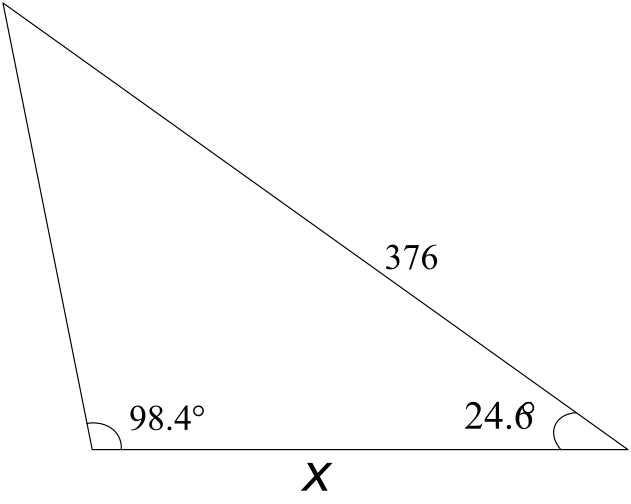
\includegraphics[ width=2.2373in, height=1.7902in,]{L4SZ2823}	}
	
	
	\item [5]    
	\setlength\fboxrule{0in}\setlength\fboxsep{0.2in}\fcolorbox[HTML]{000000}{FFFFFF}{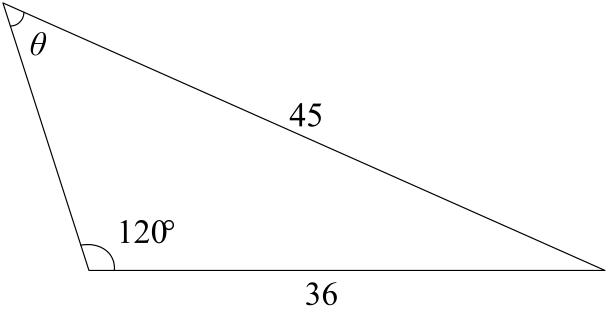
\includegraphics[ width=2.3609in, height=1.241in,]{L4SZ2824}	}
	%TCIMACRO{\TeXButton{End Two Columns}{\end {multicols}}}%
	%BeginExpansion
	\end {multicols}
	%EndExpansion
\end{description}

Solve the triangle using the Sine Rule. 


\begin{description}
	\item [7.]    
	\setlength\fboxrule{0in}\setlength\fboxsep{0.2in}\fcolorbox[HTML]{000000}{FFFFFF}{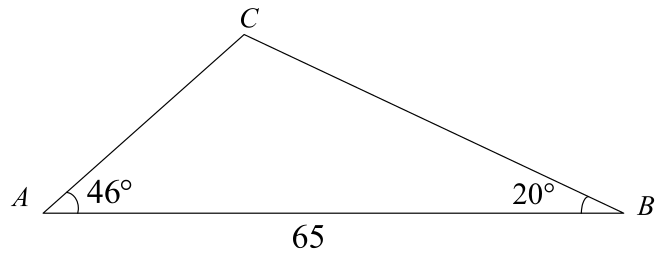
\includegraphics[ width=3.5198in, height=1.3863in,]{L4SZ2825}	}
\end{description}

%SINE RULE
Sketch each triangle and then solve the triangle using the Sine Rule. 
\begin{description}
	\item [9.] $\angle A =50 \mbox{{\ensuremath{{}^\circ}}}\text{,}$ $\angle B =68 \mbox{{\ensuremath{{}^\circ}}}\text{,}$ $c =230$ 
	
	\item [13.] $\angle B =29 \mbox{{\ensuremath{{}^\circ}}}\text{,}$ $\angle C =51 \mbox{{\ensuremath{{}^\circ}}}\text{,}$ $b =44$ 
	
	\item [23.]   
	%TCIMACRO{\TeXButton{Start Two Columns}{\columnsep =30pt
	% \begin {multicols}{2}}}%
	%BeginExpansion
	\columnsep =30pt
	\begin {multicols}{2}
	%EndExpansion
	To find the distance across a river, a surveyor chooses points $A$ and $B$, which are $200 \mbox{ft}$ apart on one side of the river. She then chooses
	a reference point $C$ on the opposite side of the river and finds that $\angle BAC \approx 82 \mbox{{\ensuremath{{}^\circ}}}$ and $\angle ABC \approx 52 \mbox{{\ensuremath{{}^\circ}}}\text{.}$  Find the approximate
	distance from $A$ to $C$. 
	
	\item    
	\setlength\fboxrule{0in}\setlength\fboxsep{0.2in}\fcolorbox[HTML]{000000}{FFFFFF}{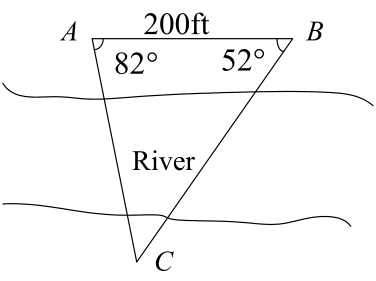
\includegraphics[ width=2.4059in, height=1.7988in,]{L4SZ2826}	}
	%TCIMACRO{\TeXButton{End Two Columns}{\end {multicols}}}%
	%BeginExpansion
	\end {multicols}
	%EndExpansion
	
	
	\item [25.]
	The path of a satellite circling the earth causes it to pass directly over two tracking stations $A$ and $B$, which are $50 \mbox{mi}$ apart. When the satellite is on one side of the
	two stations, the angle of elevation at $A$ and $B$ are measured to be $87.0 \mbox{{\ensuremath{{}^\circ}}}$ and $84.2 \mbox{{\ensuremath{{}^\circ}}}$, respectively. 
	
	\item [(a)]
	Draw a diagram. 
	
	\item [(b)] How far is the satellite from
	station $A$? 
	
	\item [(c)] How high is the satellite
	above the ground? 
	
	\columnsep =30pt
	\begin {multicols}{2}\item [27.]   
	A communication tower is located at the top of a steep hill. The angle of inclination
	of the hill is $58 \mbox{{\ensuremath{{}^\circ}}}$. A guy wire is attached to the top of the tower
	and to the ground, $100 \mbox{m}$ downhill from the base of the tower. The
	angle between the slope of the hill and the guy wire is measured as $12 \mbox{{\ensuremath{{}^\circ}}}$. Find $A C$, the length of cable required for the guy wire. 
	
	\item    
	\setlength\fboxrule{0in}\setlength\fboxsep{0.2in}\fcolorbox[HTML]{000000}{FFFFFF}{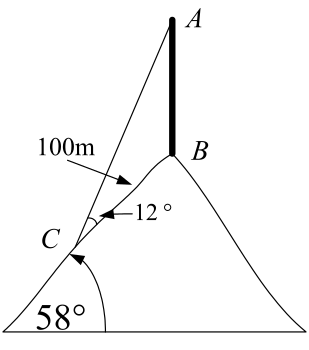
\includegraphics[ width=2.0851in, height=2.3575in,]{L4SZ2827}	}
	%TCIMACRO{\TeXButton{End Two Columns}{\end {multicols}}}%
	%BeginExpansion
	\end {multicols}
	%EndExpansion
	
	
	
	%TCIMACRO{\TeXButton{Start Two Columns}{\columnsep =30pt
	% \begin {multicols}{2}}}%
	%BeginExpansion
	\columnsep =30pt
	\begin {multicols}{2}\item [31.]
	%EndExpansion
	A water tower $30 \mbox{m}$ tall is located at the top of a hill. From
	a distance of $120 \mbox{m}$ down the hill it is observer that the angle formed between the top and
	the base of the tower is $8 \mbox{{\ensuremath{{}^\circ}}}$. Find $\angle ABC\text{,}$ the angle of inclination of the hill. 
	
	\item    
	\setlength\fboxrule{0in}\setlength\fboxsep{0.2in}\fcolorbox[HTML]{000000}{FFFFFF}{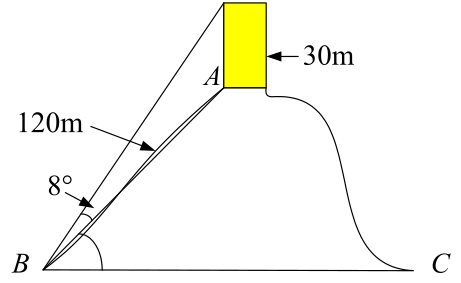
\includegraphics[ width=2.4829in, height=1.5281in,]{L4SZ2828}	}
	%TCIMACRO{\TeXButton{End Two Columns}{\end {multicols}}}%
	%BeginExpansion
	\end {multicols}
	%EndExpansion
\end{description}

\subsection{Exercises}


\begin{description}
	
	%TCIMACRO{\TeXButton{Start Two Columns}{\columnsep =30pt
	% \begin {multicols}{2}}}%
	%BeginExpansion
	\columnsep =30pt
	\begin {multicols}{2}\item [1.]
	%EndExpansion
	Use the Cosine Rule to find $x$ \\given $AC=44.3$. 
	
	\item    
	\setlength\fboxrule{0in}\setlength\fboxsep{0.2in}\fcolorbox[HTML]{000000}{FFFFFF}{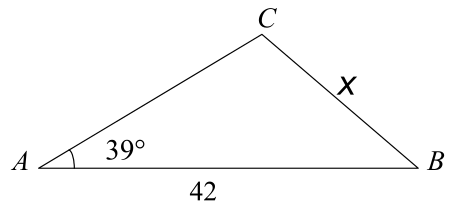
\includegraphics[ width=2.8236in, height=1.3007in,]{L4SZ282D}	}
	\vspace*{1.5cm} 
	
	\item [5.]
	Use the Cosine Rule to find $\theta $ 
	
	\item    
	\setlength\fboxrule{0in}\setlength\fboxsep{0.2in}\fcolorbox[HTML]{000000}{FFFFFF}{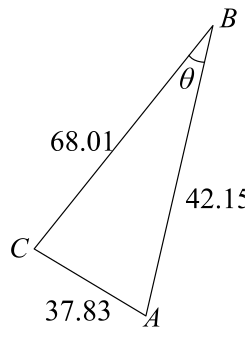
\includegraphics[ width=1.2747in, height=1.7262in,]{L4SZ282E}	}
	%TCIMACRO{\TeXButton{End Two Columns}{\end {multicols}}}%
	%BeginExpansion
	\end {multicols}
	%EndExpansion
\end{description}

Solve the triangle ABC for questions 9, 13, and 15. 


\begin{description}
	\item [9.]    
	\setlength\fboxrule{0in}\setlength\fboxsep{0.2in}\fcolorbox[HTML]{000000}{FFFFFF}{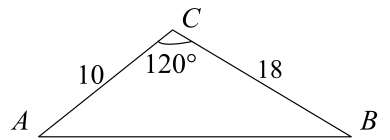
\includegraphics[ width=2.693in, height=0.9798in,]{L4SZ282F}	}
	
	
\end{description}

For questions 19 and 23 use either the Sine Rule or Cosine
Rule as appropriate. 


\begin{description}
	\item [19.]   
	%TCIMACRO{\TeXButton{Start Two Columns}{\columnsep =30pt
	% \begin {multicols}{2}}}%
	%BeginExpansion
	\columnsep =30pt
	\begin {multicols}{2}
	%EndExpansion
	
	\setlength\fboxrule{0in}\setlength\fboxsep{0.2in}\fcolorbox[HTML]{000000}{FFFFFF}{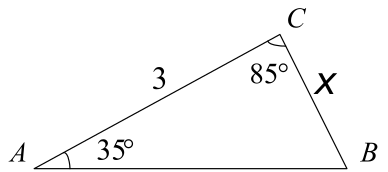
\includegraphics[ width=2.5166in, height=1.1234in,]{L4SZ282G}	}
	
	
	\item [23.]    
	\setlength\fboxrule{0in}\setlength\fboxsep{0.2in}\fcolorbox[HTML]{000000}{FFFFFF}{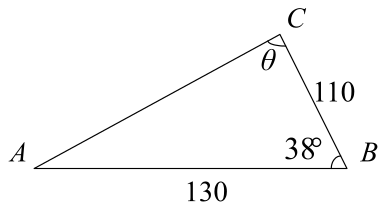
\includegraphics[ width=2.412in, height=1.3309in,]{L4SZ282H}	}
	%TCIMACRO{\TeXButton{End Two Columns}{\end {multicols}}}%
	%BeginExpansion
	\end {multicols}
	%EndExpansion
	
	
	\item [27.]
	%TCIMACRO{\TeXButton{Start Two Columns}{\columnsep =30pt
	% \begin {multicols}{2}}}%
	%BeginExpansion
	\columnsep =30pt
	\begin {multicols}{2}
	%EndExpansion
	To find the distance across a small lake, a surveyor has taken the measurements shown. Find
	the distance across the lake using this information. 
	
	\item    
	\setlength\fboxrule{0in}\setlength\fboxsep{0.2in}\fcolorbox[HTML]{000000}{FFFFFF}{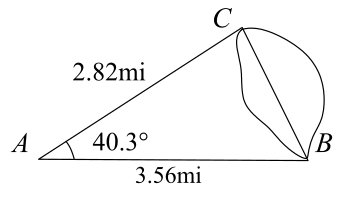
\includegraphics[ width=2.7665in, height=1.5965in,]{L4SZ282I}	}
	%TCIMACRO{\TeXButton{End Two Columns}{\end {multicols}}}%
	%BeginExpansion
	\end {multicols}
	%EndExpansion
	
	
	\item [29.]
	Two straight roads diverge at an angle of $65 \mbox{{\ensuremath{{}^\circ}}}$. Two cars leave the intersection at $2.00$ P.M., one traveling at $50 mi/\mbox{h}$ and the other at $30 mi/\mbox{h}$. How far apart are the cars at $2.30$ P.M.? 
	
	\item [31.] A pilot flies
	in a straight path for $1 \mbox{h}\; 30 \mbox{min}$. She then makes a course correction, heading $10 \mbox{{\ensuremath{{}^\circ}}}$ to the right of her original course, and flies for $2 \mbox{h}$ in the new direction. If she
	maintains a constant speed of $625 mi/\mbox{h}$ how far is she from her starting point? 
	
	\item [33.]
	A fisherman leaves his home port and heads in a direction N $70 \mbox{{\ensuremath{{}^\circ}}}$ W. he travels $30 \mbox{mi}$ and reaches Egg Island. The next day he sails N
	$10 \mbox{{\ensuremath{{}^\circ}}}$ E for $50 \mbox{mi}$, reaching Forrest Island. 
	
	\item [(a)]
	Find the distance between the fisherman's home port and Forrest Island. 
	
	\item [(b)]
	Find the bearing from Forrest Island back to his home port. 
	
	\item [35.]
	A triangular field has sides of lengths $22$, $36$, and $44$ yd. Find the largest angle. 
	
	\item [37.]
	A boy is flying two kites at the same time. He has $380 \mbox{ft}$ of line out to one kite and $420 \mbox{ft}$ of line out to the other. He estimates the angle
	between the two lines is $30 \mbox{{\ensuremath{{}^\circ}}}$. Find the approximate distance between the two
	kites. 
	
	\item [39.]   
	%TCIMACRO{\TeXButton{Start Two Columns}{\columnsep =30pt
	% \begin {multicols}{2}}}%
	%BeginExpansion
	\columnsep =30pt
	\begin {multicols}{2}
	%EndExpansion
	A steep mountain is inclined $74 \mbox{{\ensuremath{{}^\circ}}}$ to the horizontal and rises $3400 \mbox{ft}$ above the surrounding plain. A cable car is to
	be installed from a point $800 \mbox{ft}$ from the base to the top of the mountain, as shown. Find
	the shortest length of cable needed. 
	
	\item    
	\setlength\fboxrule{0in}\setlength\fboxsep{0.2in}\fcolorbox[HTML]{000000}{FFFFFF}{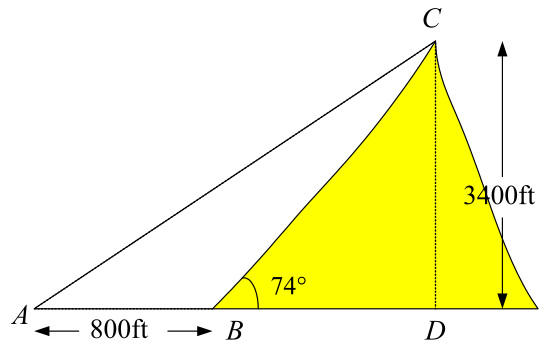
\includegraphics[ width=2.4587in, height=1.5912in,]{L4SZ282J}
	}
	%TCIMACRO{\TeXButton{End Two Columns}{\end {multicols}}}%
	%BeginExpansion
	\end {multicols}
	%EndExpansion
\end{description}


\begin{description}
	\item [41.] Three circles of radii $4$, $5$, and $6 \mbox{cm}$ respectively are mutually tangent. Find the area
	enclosed between the circles. 
	
	\item \qquad \qquad \qquad \qquad
	\setlength\fboxrule{0in}\setlength\fboxsep{0.2in}\fcolorbox[HTML]{000000}{FFFFFF}{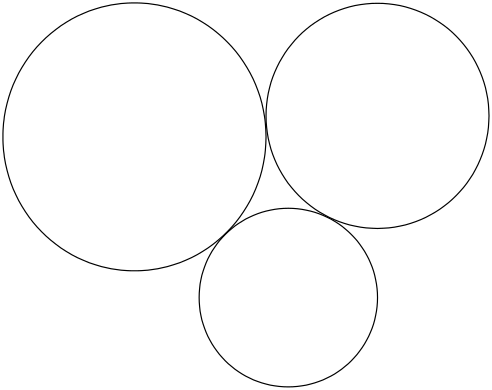
\includegraphics[ width=3.3269in, height=2.6394in,]{L4SZ282K}
	}
	
	
	
	%TCIMACRO{\TeXButton{Start Two Columns}{\columnsep =30pt
	% \begin {multicols}{2}}}%
	%BeginExpansion
	\columnsep =30pt
	\begin {multicols}{2}\item [43.]   
	%EndExpansion
	A surveyor wishes to find the distance between two points $A$ and $B$ on the opposite side of a river. on her side of the river she chooses two points
	$C$ and $D$ that are $20 \mbox{m}$ apart and measures the angles shown. Find
	the distance between $A$ and $B\text{.}$ 
	
	\item    
	\setlength\fboxrule{0in}\setlength\fboxsep{0.2in}\fcolorbox[HTML]{000000}{FFFFFF}{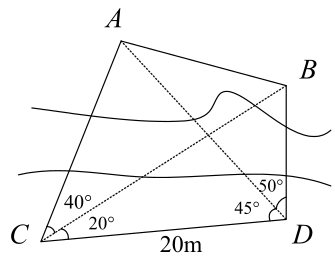
\includegraphics[ width=2.5028in, height=1.9995in,]{L4SZ282L}
	}
	%TCIMACRO{\TeXButton{End Two Columns}{\end {multicols}}}%
	%BeginExpansion
	\end {multicols}
	%EndExpansion
	
	
	\item [45.]
	Land in downtown Columbia is valued at $ \$20$ a square foot. What is the value of a triangular lot with sides of lengths $112$, $148$, and $190 \mbox{ft}$? \end{description}

\subsection{Exercises}
Graph the functions by hand. 

\begin{description}
	\item [1.]   
	%TCIMACRO{\TeXButton{Start Two Columns}{\columnsep =30pt
	% \begin {multicols}{2}}}%
	%BeginExpansion
	\columnsep =30pt
	\begin {multicols}{2}
	%EndExpansion
	$y =1 +\sin  x$ %soln file {L4SZ270N}
	
	\item [3.] $y =1 -\cos  x$ %soln file {L4SZ270O}
	%TCIMACRO{\TeXButton{End Two Columns}{\end {multicols}}}%
	%BeginExpansion
	\end {multicols}
	%EndExpansion
	
	\columnsep =30pt
	\begin {multicols}{2}
	\item [5.]
	%TCIMACRO{\TeXButton{Start Two Columns}{\columnsep =30pt
	% \begin {multicols}{2}}}%
	%BeginExpansion
	
	%EndExpansion
	$y = -2 \sin  x$ %soln file {L4SZ270P}
	
	\item [7.] $y =4 -2 \cos  x$%soln file  {L4SZ270Q}
	%TCIMACRO{\TeXButton{End Two Columns}{\end {multicols}}}%
	%BeginExpansion
	\end {multicols}
	%EndExpansion
	
	
	\item [9.]
	$y =\left \vert \cos  x\right \vert $%soln file {L4SZ270R}
 \end{description}

Find the amplitude
and period of the function and sketch its graph. 


\begin{description}
	\item [11.]   
	%TCIMACRO{\TeXButton{Start Two Columns}{\columnsep =30pt
	% \begin {multicols}{2}}}%
	%BeginExpansion
	\columnsep =30pt
	\begin {multicols}{2}
	%EndExpansion
	$y =\cos  4 x$ 
	
	\item [13.] $y =3 \sin  3 x$ 
	%TCIMACRO{\TeXButton{End Two Columns}{\end {multicols}}}%
	%BeginExpansion
	\end {multicols}
	%EndExpansion
	
	
	\item [15.]
	%TCIMACRO{\TeXButton{Start Two Columns}{\columnsep =30pt
	% \begin {multicols}{2}}}%
	%BeginExpansion
	\columnsep =30pt
	\begin {multicols}{2}
	%EndExpansion
	$y =10 \sin  \frac{1}{2} x$ 
	
	\item [17.] $y = -\cos  \frac{1}{3} x$ 
	%TCIMACRO{\TeXButton{End Two Columns}{\end {multicols}}}%
	%BeginExpansion
	\end {multicols}
	%EndExpansion
	
	
	\item [19.]
	$y =3 \cos  3 \pi  x$ \end{description}

Find the amplitude, period and phase shift of the function,
and graph one complete period. 


\begin{description}
	
	%TCIMACRO{\TeXButton{Start Two Columns}{\columnsep =30pt
	% \begin {multicols}{2}}}%
	%BeginExpansion
	\columnsep =30pt
	\begin {multicols}{2}	\item [21.]  
	%EndExpansion
	$y =\cos  \left (x -\frac{\pi }{2}\right )$ 
	
	\item [23.] $y = -\sin  \left (x -\frac{\pi }{6}\right )$ 
	%TCIMACRO{\TeXButton{End Two Columns}{\end {multicols}}}%
	%BeginExpansion
	\end {multicols}
	%EndExpansion
	
	
	\item [25.]
	%TCIMACRO{\TeXButton{Start Two Columns}{\columnsep =30pt
	% \begin {multicols}{2}}}%
	%BeginExpansion
	\columnsep =30pt
	\begin {multicols}{2}
	%EndExpansion
	$y =5 \cos  \left (3 x -\frac{\pi }{4}\right )$ 
	
	\item [27.] $y =2 \sin  \left (\frac{2}{3} x -\frac{\pi }{6}\right )$ 
	%TCIMACRO{\TeXButton{End Two Columns}{\end {multicols}}}%
	%BeginExpansion
	\end {multicols}
	%EndExpansion
	
	
	\item [29.]
	%TCIMACRO{\TeXButton{Start Two Columns}{\columnsep =30pt
	% \begin {multicols}{2}}}%
	%BeginExpansion
	\columnsep =30pt
	\begin {multicols}{2}
	%EndExpansion
	$y =3 \cos  \pi  \left (x +\frac{1}{2}\right )$ 
	
	\item [31.] $y = -\frac{1}{2} \cos  \left (2 x -\frac{\pi }{3}\right )$ 
	%TCIMACRO{\TeXButton{End Two Columns}{\end {multicols}}}%
	%BeginExpansion
	\end {multicols}
	%EndExpansion
	
	
	\item [33.]
	$y =\sin  \left (3 x +\pi \right )$ \end{description}

Use Desmos to complete the following questions: 

\begin{description}\item [41.]
	
	%TCIMACRO{\TeXButton{Start Two Columns}{\columnsep =30pt
	% \begin {multicols}{2}}}%
	%BeginExpansion
	\columnsep =30pt
	\begin {multicols}{2}
	%EndExpansion
	$f (x) =\cos  100 x$ 
	
	\item [43.] $f (x) =\sin  \genfrac{(}{)}{}{}{x}{40}$ 
	%TCIMACRO{\TeXButton{End Two Columns}{\end {multicols}}}%
	%BeginExpansion
	\end {multicols}
	%EndExpansion
	
	
	\item [47.]
	$y =e^{\sin  20 x}$ \end{description}

Graph $f$, $g$ and $f +g$ on a common screen to illustrate graphical addition. 

Graph the three functions on a common screen. How
are the graphs related? 

\begin{description}
	\item [55.]   
	%TCIMACRO{\TeXButton{Start Two Columns}{\columnsep =30pt
	% \begin {multicols}{2}}}%
	%BeginExpansion
	\columnsep =30pt
	\begin {multicols}{2}
	%EndExpansion
	$y =x^{2} ,\text{\quad \quad }y = -x^{2} ,\text{\quad \quad }y =x^{2} \sin  x$ 
	
	\item [57.] $y =e^{x} ,\text{\quad \quad }y = -e^{x} ,\text{\quad \quad }y =e^{x} \sin  5 \pi  x$ 
	%TCIMACRO{\TeXButton{End Two Columns}{\end {multicols}}}%
	%BeginExpansion
	\end {multicols}
	%EndExpansion
\end{description}
Find the values of the trigonometric ratios.
\ If possible give the exact value; otherwise use a calculator to find an approximate value correct to 5 decimal
places. 


\begin{description}
	\columnsep =30pt
	\begin {multicols}{2}
	\item [9.]   
	%TCIMACRO{\TeXButton{Start Two Columns}{\columnsep =30pt
	% \begin {multicols}{2}}}%
	%BeginExpansion
	%EndExpansion
	(a) $\sin  1.1\text{\quad \quad }$(b) $\cos  1.1$ 
	
	\item [10.] (a) $\cos  \frac{\pi }{5}\text{\quad \quad }$(b) $\cos  \left ( -\frac{\pi }{5}\right )$ 
	%TCIMACRO{\TeXButton{End Two Columns}{\end {multicols}}}%
	%BeginExpansion
	\end {multicols}
	%EndExpansion
	
	
	\item [21.]
	Given $\sin  t =\frac{5}{13}$ and $\cos  t = -\frac{12}{13}$ find $\tan  t$ 
\end{description}

